% ============================================================================
%  M.Sc. Thesis  --  paper-style scaffold
%  Systemic mapping of cytokine signalling cascades from single-cell snapshots
%
%  Build:  pdflatex thesis  &&  bibtex thesis  &&  pdflatex thesis  &&  pdflatex thesis
%  (or just run latexmk -pdf thesis.tex ; see README.md)
%
%  This file is a SKELETON: preamble + section titles only.
%  Write the content yourself under each "% >>> write here" marker.
% ============================================================================
\documentclass[11pt,a4paper]{article}

% ---- page geometry ---------------------------------------------------------
\usepackage[margin=1in]{geometry}
\usepackage[english]{babel}

% ---- encoding & fonts ------------------------------------------------------
\usepackage[T1]{fontenc}
\usepackage[utf8]{inputenc}
% lmodern is in every TeX install. For a Times-like "paper" look instead,
% install the newtx package and swap to the two commented lines below.
\usepackage{lmodern}
% \usepackage{newtxtext}
% \usepackage{newtxmath}
\usepackage{microtype}            % subtle spacing/kerning improvements

% ---- math ------------------------------------------------------------------
\usepackage{amsmath,amssymb,amsthm}
\usepackage{bm}

% ---- tables, figures, graphics --------------------------------------------
\usepackage{graphicx}
\graphicspath{{figures/}}
\usepackage{booktabs}
\usepackage[table]{xcolor}
\usepackage{caption}
\usepackage{subcaption}
\usepackage{float}
\usepackage{tikz}   % schematic figures (default arrow tips; arrows.meta not installed)
% For pgfplots data figures (as in reports/method_summary), also:
% tlmgr install pgfplots ; then \usepackage{pgfplots}\pgfplotsset{compat=1.18}

% ---- lists & layout --------------------------------------------------------
\usepackage{enumitem}
\usepackage{titlesec}
\usepackage{setspace}
\onehalfspacing
\usepackage{parskip}   % gap between paragraphs, no first-line indent (block style)

% ---- bibliography ----------------------------------------------------------
\usepackage[numbers,sort&compress]{natbib}
\bibliographystyle{unsrtnat}

% ---- cross-refs & links (load hyperref late) ------------------------------
\usepackage[colorlinks=true,linkcolor=black,citecolor=black,urlcolor=blue]{hyperref}
% Smart cross-references (\cref). Install with: tlmgr install cleveref
% \usepackage{cleveref}

% ---- handy macros (extend as you write) -----------------------------------
\newcommand{\crossasym}{\texttt{cross\_asym}}
\newcommand{\todo}[1]{\textcolor{red}{[TODO: #1]}}
\newcommand{\rev}[1]{#1}  % cleared: new text no longer marked; kept as a no-op wrapper

% ============================================================================
\begin{document}

% ----------------------------------------------------------------------------
%  TITLE PAGE
% ----------------------------------------------------------------------------
\begin{titlepage}
\centering
\vspace*{2cm}

{\LARGE\bfseries Systemic Mapping of Cytokine Signalling Cascades\\[0.3em]
from Single-Cell Snapshots via Multiple-Instance-Learning Dynamics\par}

\vspace{2cm}
{\large Yam Arieli\par}

\vspace{2cm}
{\large A thesis submitted in partial fulfilment\\
of the requirements for the degree of\\
Master of Science\par}

\vspace{1.5cm}
{\large Advisor: \todo{advisor name}\par}
\vspace{0.5cm}
{\large \todo{department / school}\\
The Hebrew University of Jerusalem\par}

\vfill
{\large \today\par}
\end{titlepage}

% ----------------------------------------------------------------------------
%  FRONT MATTER
% ----------------------------------------------------------------------------
\pagenumbering{roman}

\begin{abstract}
While Immune cells communicate via cytokine signalling cascades that span over time, most of the time we have only single-cell snapshots of the system. In this work, we present a novel approach to infer the dynamics of cytokine signalling cascades from single-cell data using the dynamics of model training to capture the temporal evolution of the system. We demonstrate that our approach can reconstruct the dynamics of cytokine signalling cascades from single-cell snapshots, providing new insights into the temporal evolution of immune cell communication.
\end{abstract}

\newpage
\section*{Acknowledgements}
% >>> write here

\newpage
\tableofcontents
\newpage

% ----------------------------------------------------------------------------
%  MAIN MATTER
% ----------------------------------------------------------------------------
\pagenumbering{arabic}
\setcounter{page}{1}

\section{Introduction}
\label{sec:introduction}
% >>> write here

\section{Background}
\label{sec:background}
% >>> write here

\subsection{Biological background}
Immune cells communicate largely through cytokines: secreted proteins that carry a signal from a producing cell to any cell bearing the matching receptor.
The signal reshapes the cell's behavior: it can drive the cell to proliferate, to differentiate into a new state, to survive or undergo death, or to migrate.
Each of these behaviors is driven by a change in gene expression, so it leaves a transcriptional trace in the cell's RNA. How fully that trace captures the behavior varies: cell identity and proliferation are written clearly, whereas migration registers only faintly.

Crucially, part of the response can be the up-regulation of cytokine genes: a cell that receives one cytokine may, as part of its program, secrete another.
Chaining these steps produces a signalling cascade, cytokine A leading to B leading to C, a process that by its nature unfolds in a fixed temporal order.
Because the responding population is a mixture of distinct cell types, and each cytokine acts only where its receptor is present, every step of a cascade is confined to particular cell types.
This makes certain cell types relays: an intermediary responds to the upstream cytokine and produces the downstream one, carrying the cascade from one signal to the next.

Mapping this wiring matters because cytokine cascades sit at the centre of both healthy immune coordination and its failures, and many therapies act by targeting a single cytokine within them. Yet knowing where a therapy should act depends on more than a list of couplings: it requires knowing which cytokine is upstream, and through which relay, turning a static catalogue of immune responses into a map of how signals actually flow. That direction is exactly what today usually demands perturbation or time-course experiments; recovering it instead from a single static snapshot, the aim of this work, would make the knowledge far cheaper and open it to the many single-cell datasets that already exist.
% >>> write here

\subsection{Computational background}
\label{sec:comp-background}
Single-cell RNA sequencing measures each cell individually, representing it as a high-dimensional vector of gene-expression values.
What we know, however, is not the state of each cell but only which stimulus was applied to the sample as a whole; the individual cells carry no labels of their own.

Learning from such data, where a label describes a bag of instances rather than any one of them, is the problem studied under the name Multiple Instance Learning (MIL).
The approach adopted here is embedding-based MIL: each instance is mapped to a learned representation, the representations are aggregated into a single bag vector, and the label is predicted from that vector.
A bag of cells is a set, not a sequence: its cells have no meaningful order, so the aggregation must return the same prediction however they are arranged. It must also handle that only some cells respond informatively to the stimulus while many are uninformative bystanders. Attention-based MIL meets both needs: it aggregates the cells by a learned weighted sum, which is invariant to their order, while the learned weights let the model concentrate on the informative cells instead of diluting them in a plain average. A further benefit is interpretability: because each cell carries an explicit weight, the attention distribution shows which cells the model relied on to identify the stimulus.
% >>> write here

\section{Related Work}
\label{sec:related-work}
% >>> write here

\section{Methods}
\label{sec:methods}
% >>> write here

\subsection{The idea}
\label{sec:methods-idea}
Our approach is built on two premises. The first is that every cytokine leaves a distinctive transcriptional signature, a set of genes it characteristically induces in the cells that respond to it. The second is that these signatures reveal cascades: the presence of cytokine Y's signature within the response to cytokine X indicates that X drives Y.

\subsubsection{Claim 1: each cytokine induces a distinctive signature}
\label{sec:claim-signature}
We define a cytokine's signature $S_X$ as the $k$ genes that, together, make its response most separable from the control baseline \citep{golub1999molecular}. Formally,
\[
  S_X \;=\; \operatorname*{arg\,max}_{\substack{G\subseteq\mathcal{G}\\ |G|=k}}\ \operatorname{acc}_{X}(G),
\]
where $\mathcal{G}$ is the set of all genes, $\operatorname{acc}_{X}(G)$ is the accuracy of a classifier that tells $X$ from the control using only the genes $G$, and $k$ fixes the signature's size (we choose $k=50$ in our experiments).
Recent work makes this concrete: a single-cell dictionary of immune responses recorded a distinct signature for dozens of cytokines, confirming that their responses are separable at the transcriptional level \citep{cui2024dictionary}.
The distinctiveness is not accidental: because a cytokine acts through its own receptor and a specific downstream pathway, it engages a particular set of transcription factors, and so induces its own target genes.
Throughout, a cytokine's signature is measured in the responding cells' gene expression, not in the cytokine itself; the molecule is invisible to us, and only its transcriptional footprint is seen.

\subsubsection{Claim 2: asymmetric cross-presence of signatures reveals direction}
\label{sec:claim-direction}
If X lies upstream of Y, a sample given only X still generates Y internally: relay cells produce Y and others respond, imprinting Y's signature onto the X condition.
That a stimulated sample generates such secondary responses is well documented: type I interferon induced downstream of Toll-like receptor activation acts back on the same and neighbouring cells to induce its own signature \citep{gautier2005type}, and single-cell measurements have resolved these paracrine cascades directly \citep{xue2015single}.
The direction comes from an asymmetry: cells given X carry both X's own signature and the induced Y signature, while cells given Y carry mainly their own. This is because X is not produced downstream of Y, so little of X's signature appears in the Y condition. Comparing how much of each signature appears in the other condition therefore points from upstream to downstream.

\begin{figure}[H]
\centering
% ---------- panel (a): the geometry ----------
\begin{minipage}[c]{0.46\textwidth}
\centering
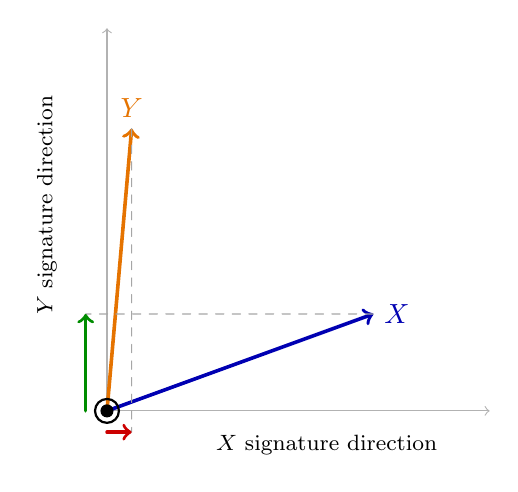
\begin{tikzpicture}[scale=0.9, line cap=round]
  % axes (abstract gene space)
  \draw[->, gray!60] (0,0) -- (5.4,0);
  \draw[->, gray!60] (0,0) -- (0,5.4);
  \node[below] at (3.1,-0.2) {\footnotesize $X$ signature direction};
  \node[rotate=90] at (-0.85,2.9) {\footnotesize $Y$ signature direction};
  % equal-length response vectors
  \coordinate (O) at (0,0);
  \coordinate (X) at (20:4);
  \coordinate (Y) at (85:4);
  \draw[->, line width=1.3pt, blue!70!black]   (O) -- (X) node[right] {$X$};
  \draw[->, line width=1.3pt, orange!90!black] (O) -- (Y) node[above] {$Y$};
  % orthogonal projections onto the OTHER cytokine's direction (dashed guides)
  \draw[dashed, gray!70] (X) -- (-0.3, {4*sin(20)});
  \draw[dashed, gray!70] (Y) -- ({4*cos(85)}, -0.3);
  % projection-magnitude arrows
  \draw[->, green!55!black, line width=1.2pt] (-0.3,0) -- (-0.3, {4*sin(20)});
  \draw[->, red!80!black,   line width=1.2pt] (0,-0.3) -- ({4*cos(85)}, -0.3);
  % reference symbol at the origin
  \filldraw[black] (O) circle (2.4pt);
  \draw[black, line width=0.8pt] (O) circle (4.8pt);
\end{tikzpicture}\\[2pt]
{\footnotesize (a)}
\end{minipage}\hfill
% ---------- panel (b): the reading ----------
\begin{minipage}[c]{0.5\textwidth}
\centering
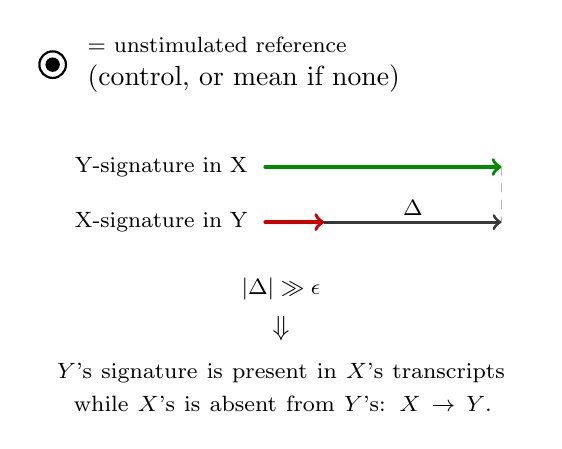
\begin{tikzpicture}[line cap=round]
  % reference-symbol legend
  \filldraw[black] (0,4.7) circle (2.4pt);
  \draw[black, line width=0.8pt] (0,4.7) circle (4.8pt);
  \node[right, align=left] at (0.32,4.7) {\footnotesize $=$ unstimulated reference\\(control, or mean if none)};
  % the two magnitudes as bars, same start
  \node[left] at (2.6,3.4) {\footnotesize Y-signature in X};
  \node[left] at (2.6,2.7) {\footnotesize X-signature in Y};
  \draw[->, green!55!black, line width=1.3pt] (2.7,3.4) -- (5.7,3.4);
  \draw[->, red!80!black,   line width=1.3pt] (2.7,2.7) -- (3.45,2.7);
  % delta: from the red tip to the green tip's x-position
  \draw[dashed, gray!55] (5.7,3.4) -- (5.7,2.7);
  \draw[->, gray!45!black, line width=1.1pt] (3.45,2.7) -- (5.7,2.7);
  \node[above] at (4.575,2.66) {\footnotesize $\Delta$};
  % relation and conclusion
  \node at (2.9,1.85) {\footnotesize $\lvert \Delta \rvert \gg \epsilon$};
  \node at (2.9,1.35) {$\Downarrow$};
  \node[align=center, text width=6.2cm] at (2.9,0.6)
    {\footnotesize $Y$'s signature is present in $X$'s transcripts while $X$'s is absent from $Y$'s: $X \to Y$.};
\end{tikzpicture}\\[2pt]
{\footnotesize (b)}
\end{minipage}
\caption{\textbf{The direction cue as an asymmetry in signature space.} \textbf{(a)} The
two axes are the $X$ and $Y$ signature directions, the equal-weighted average over each
cytokine's signature genes, within the full gene space; the ringed dot at the origin is the
unstimulated reference. The two equal-length vectors are the \emph{full transcriptional
responses} to stimulus $X$ and to stimulus $Y$, and each is projected onto both signature
directions. The dashed guides give each response's orthogonal projection onto the
\emph{other} cytokine's direction: the $X$ response onto the $Y$ direction (green) and the
$Y$ response onto the $X$ direction (red). \textbf{(b)} These two cross-projections compared
directly: the $X$ response's component in the $Y$ direction (green, ``$Y$-signature in
$X$'') far exceeds the $Y$ response's component in the $X$ direction (red, ``$X$-signature
in $Y$''); their difference
$\Delta$ is large ($\lvert\Delta\rvert \gg \epsilon$), read as the direction $X \to Y$.}
\label{fig:asymmetry}
\end{figure}
% >>> write here

\subsection{Sub-goals}
\label{sec:methods-subgoals}
The method decomposes into three sub-goals, all of which must be achieved without injecting prior knowledge and from a single snapshot in time, the two constraints set out in the Introduction (Section~\ref{sec:introduction}).
\begin{enumerate}
\item \textbf{Discover signatures.} Obtain, for each cytokine, a data-driven signature $S_X$: the genes most informative for identifying its response.
\item \textbf{Find coupling.} Identify cytokine pairs whose signatures are related, marking a shared-biology link, without yet assigning a direction.
\item \textbf{Assign direction.} Within each coupled pair, determine which cytokine is upstream, from the asymmetric cross-presence of the two signatures.
\end{enumerate}

\subsection{Data}
\label{sec:methods-data}
\rev{The method works from a single snapshot, the gene expression of many individual cells captured at one moment rather than followed over time.}
\rev{Each cell is tagged with the condition it was under: most often the cytokine applied to it, but equally a cell state, a timepoint, or a disease grade.}
\rev{One of these conditions is a control, an untreated or baseline state that the others are compared to.}
\rev{Two further labels travel with each cell: the donor it came from, which fixes the biological replicate, and its cell type, which lets like be compared with like.}

\rev{Rather than one cell at a time, the method takes a whole set of cells sampled together, a matrix of cells by genes, and predicts a single condition for the set.}
\rev{This mirrors the biology: the cells of one sample sat together under the same condition, so the set as a whole, not any single cell, is what the condition acted on.}
\rev{In practice, though, a donor and condition yield only one tube of cells, a single example where the model needs many.}
\rev{So we draw many smaller bags from the one tube at random, each stratified by cell type; these stochastic sub-samples are the pseudo-tubes (Figure~\ref{fig:pseudotube}).}

\begin{figure}[H]
\centering
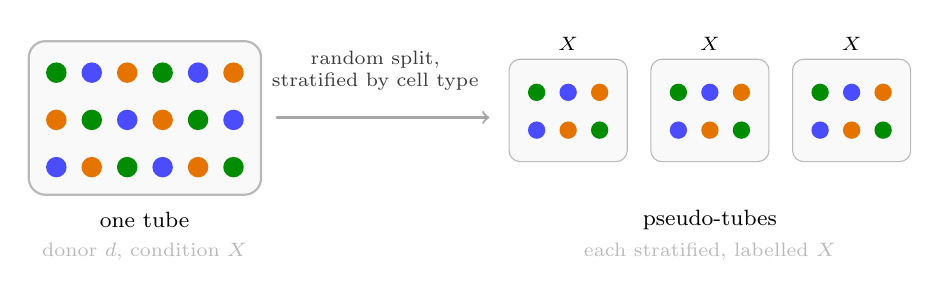
\begin{tikzpicture}[line cap=round]
  % ---------------- one tube (left) ----------------
  \fill[gray!5, rounded corners=6pt] (0.1,0.2) rectangle (3.05,2.15);
  \foreach \x/\y in {0.45/0.55,1.8/0.55,1.35/1.15,2.7/1.15,0.9/1.75,2.25/1.75}
    \fill[blue!70] (\x,\y) circle (0.13);
  \foreach \x/\y in {0.9/0.55,2.25/0.55,0.45/1.15,1.8/1.15,1.35/1.75,2.7/1.75}
    \fill[orange!90!black] (\x,\y) circle (0.13);
  \foreach \x/\y in {1.35/0.55,2.7/0.55,0.9/1.15,2.25/1.15,0.45/1.75,1.8/1.75}
    \fill[green!55!black] (\x,\y) circle (0.13);
  \draw[rounded corners=6pt, thick, gray!55] (0.1,0.2) rectangle (3.05,2.15);
  \node[font=\footnotesize] at (1.57,-0.12) {one tube};
  \node[font=\scriptsize, gray!55] at (1.57,-0.52) {donor $d$, condition $X$};

  % ---------------- split arrow ----------------
  \draw[->, thick, gray!70] (3.25,1.18) -- (5.95,1.18);
  \node[font=\scriptsize, align=center, gray!45!black] at (4.5,1.78)
    {random split,\\stratified by cell type};

  % ---------------- pseudo-tubes (right) ----------------
  \foreach \X in {6.2,8.0,9.8}{
    \fill[gray!5, rounded corners=4pt] (\X,0.62) rectangle (\X+1.5,1.92);
    \fill[blue!70]         (\X+0.35,1.02) circle (0.11);
    \fill[orange!90!black] (\X+0.75,1.02) circle (0.11);
    \fill[green!55!black]  (\X+1.15,1.02) circle (0.11);
    \fill[green!55!black]  (\X+0.35,1.5)  circle (0.11);
    \fill[blue!70]         (\X+0.75,1.5)  circle (0.11);
    \fill[orange!90!black] (\X+1.15,1.5)  circle (0.11);
    \draw[rounded corners=4pt, gray!55] (\X,0.62) rectangle (\X+1.5,1.92);
    \node[font=\scriptsize] at (\X+0.75,2.12) {$X$};
  }
  \node[font=\footnotesize] at (8.75,-0.12) {pseudo-tubes};
  \node[font=\scriptsize, gray!55] at (8.75,-0.52) {each stratified, labelled $X$};
\end{tikzpicture}
\caption{\rev{\textbf{Building pseudo-tubes.} The single tube of cells obtained from one
donor under one condition (left; dot colour $=$ cell type) is split at random, stratified
by cell type, into several smaller pseudo-tubes (right). Each pseudo-tube keeps the tube's
cell-type mix and carries the same condition label $X$; these stochastic sub-samples are
the examples the model is trained on.}}
\label{fig:pseudotube}
\end{figure}

\subsection{Discovering cytokine signatures}
\label{sec:methods-signatures}
% >>> write here (opening: goal + strategy + "what the model is NOT" disclaimer)

\subsubsection{Strategy}
\label{sec:sig-strategy}
Rather than list signature genes by hand, we recover them from a trained classifier: if a model can identify a cytokine from its cells, the genes it relies on are, by construction, that cytokine's most informative genes.
The model is therefore only a means: it is trained to predict the stimulus label and nothing else, and once the signatures are read out of it, it is discarded; it does not predict cascades, nor does it output signatures directly.
What remains is to specify the classifier: its architecture (Section~\ref{sec:sig-architecture}), its training (Section~\ref{sec:sig-training}), and how the signatures are extracted from it (Section~\ref{sec:sig-extraction}).

\subsubsection{Architecture}
\label{sec:sig-architecture}
The classifier maps a pseudo-tube (Section~\ref{sec:methods-data}) to a stimulus prediction with an embedding-based multiple-instance-learning (MIL) model, built from three components in sequence: a per-cell encoder, an attention layer that aggregates the cells, and a linear classifier. In MIL the label is attached to a whole bag of instances rather than to any one of them (Section~\ref{sec:comp-background}); here the bag is the pseudo-tube and the instances are its cells, so the model must identify the stimulus from the cells taken together.

The encoder processes one cell at a time, mapping its gene-expression vector to a compact embedding of that cell's type. We train it to classify cell type for two reasons. First, cell identity is usually the strongest signal in single-cell expression \citep{kang2018multiplexed,luecken2019current,srivatsan2020massively}, so capturing it first frees the rest of the model to attend to the subtler, stimulus-specific differences rather than rediscovering what each cell is (Figure~\ref{fig:umap}). Second, cell type is the natural coordinate of the response: each cell type reacts to a stimulus in its own way, so an embedding organised by cell type gives a biologically meaningful space in which those effects can be read.

The stimulus acts on the tube as a whole and only some of its cells respond, so the evidence for which stimulus was applied lies in the cells collectively; we therefore need to aggregate all cells of a pseudo-tube into a single representation.
The attention layer aggregates by a weighted sum whose weights are learned: the model decides how much each cell contributes to the tube representation.
Simple alternatives fall short: mean-pooling drowns the few responding cells in a majority of bystanders, and max-pooling collapses the tube to a single cell and loses the distributed pattern; only a learned weighting can adapt to a responsive subset whose size and identity change with the stimulus.
This weighted-sum pooling is permutation-invariant, as the set structure of the tube requires (Section~\ref{sec:comp-background}), and follows the attention-based MIL formulation of \citet{ilse2018attention}.
The attention receives the encoder's output, so it selects and weights cells within the cell-type latent space: relevance is judged by what each cell is, and stimulus effects are read in cell-type features rather than raw genes. The resulting tube vector is handed to the classifier.

The final component is a linear classifier: it maps the tube vector to a probability over the stimulus classes. We keep the classifier linear on purpose: this places the model's expressive power in the encoder and attention, and leaves the stimulus decision a transparent function of the tube vector.

\begin{figure}[H]
\centering
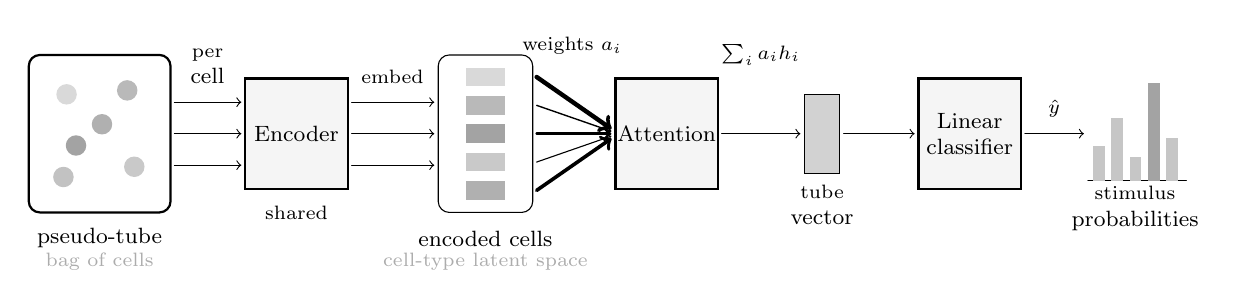
\begin{tikzpicture}[font=\footnotesize, line cap=round]
  % ---------- 1. pseudo-tube ----------
  \draw[rounded corners, thick] (-0.9,-1.0) rectangle (0.9,1.0);
  \fill[gray!30] (-0.42,0.50) circle (0.13);
  \fill[gray!55] (0.35,0.55)  circle (0.13);
  \fill[gray!72] (-0.30,-0.15) circle (0.13);
  \fill[gray!42] (0.44,-0.42) circle (0.13);
  \fill[gray!62] (0.03,0.12)  circle (0.13);
  \fill[gray!48] (-0.46,-0.55) circle (0.13);
  \node at (0,-1.33) {pseudo-tube};
  \node[gray!65] at (0,-1.63) {\scriptsize bag of cells};
  % ---------- arrows: tube -> encoder (per cell) ----------
  \foreach \y in {0.4,0,-0.4} {\draw[->] (0.95,\y) -- (1.8,\y);}
  \node[align=center] at (1.37,0.86) {\scriptsize per\\cell};
  % ---------- 2. encoder ----------
  \draw[thick, fill=gray!8] (1.85,-0.7) rectangle (3.15,0.7);
  \node at (2.5,0) {Encoder};
  \node at (2.5,-1.0) {\scriptsize shared};
  % ---------- arrows: encoder -> encoded ----------
  \foreach \y in {0.4,0,-0.4} {\draw[->] (3.2,\y) -- (4.25,\y);}
  \node at (3.72,0.72) {\scriptsize embed};
  % ---------- 3. encoded cells ----------
  \draw[rounded corners] (4.3,-1.0) rectangle (5.5,1.0);
  \foreach \y/\g in {0.72/30, 0.36/55, 0.0/72, -0.36/42, -0.72/62}
    {\fill[gray!\g] (4.65,{\y-0.12}) rectangle (5.15,{\y+0.12});}
  \node at (4.9,-1.33) {encoded cells};
  \node[gray!65] at (4.9,-1.63) {\scriptsize cell-type latent space};
  % ---------- converging arrows: encoded -> attention (weights a_i) ----------
  \draw[->, line width=1.6pt] (5.55,0.72)  -- (6.5,0.06);
  \draw[->, line width=0.5pt] (5.55,0.36)  -- (6.5,0.03);
  \draw[->, line width=1.0pt] (5.55,0.0)   -- (6.5,0.0);
  \draw[->, line width=0.4pt] (5.55,-0.36) -- (6.5,-0.03);
  \draw[->, line width=1.3pt] (5.55,-0.72) -- (6.5,-0.06);
  \node at (6.0,1.12) {\scriptsize weights $a_i$};
  % ---------- 4. attention ----------
  \draw[thick, fill=gray!8] (6.55,-0.7) rectangle (7.85,0.7);
  \node at (7.2,0) {Attention};
  % ---------- arrow: attention -> tube vector ----------
  \draw[->] (7.9,0) -- (8.9,0);
  \node at (8.4,1.0) {\scriptsize $\sum_i a_i h_i$};
  % ---------- 5. tube vector ----------
  \fill[gray!35] (8.95,-0.5) rectangle (9.4,0.5);
  \draw (8.95,-0.5) rectangle (9.4,0.5);
  \node[align=center] at (9.175,-0.9) {\scriptsize tube\\vector};
  % ---------- arrow: tube vector -> classifier ----------
  \draw[->] (9.45,0) -- (10.35,0);
  % ---------- 6. classifier ----------
  \draw[thick, fill=gray!8] (10.4,-0.7) rectangle (11.7,0.7);
  \node[align=center] at (11.05,0) {Linear\\classifier};
  % ---------- arrow: classifier -> probabilities ----------
  \draw[->] (11.75,0) -- (12.5,0);
  \node at (12.12,0.32) {\scriptsize $\hat{y}$};
  % ---------- 7. class-probability bar ----------
  \draw (12.55,-0.6) -- (13.8,-0.6);
  \foreach \i/\h/\g in {0/0.45/45, 1/0.80/45, 2/0.30/45, 3/1.25/72, 4/0.55/45}
    {\fill[gray!\g] ({12.62+\i*0.23},-0.6) rectangle ({12.62+\i*0.23+0.15},{-0.6+\h});}
  \node[align=center] at (13.15,-0.95) {\scriptsize stimulus\\probabilities};
\end{tikzpicture}
\caption{\textbf{The signature-discovery model.} A pseudo-tube (a bag of cells, each a
gene-expression vector) is processed left to right. The encoder embeds \emph{each cell}
independently (parallel arrows) into the cell-type latent space; the attention layer then
takes \emph{all} cell embeddings \emph{together} (converging arrows), weights them by
$a_i$ and sums them into a single tube vector; the linear classifier maps that vector to a
probability over the stimulus classes. The model outputs only a stimulus label; the
per-cytokine signature is extracted from the trained model afterwards
(Section~\ref{sec:sig-extraction}), and the model is then discarded.}
\label{fig:model}
\end{figure}

\subsubsection{Training}
\label{sec:sig-training}
We train in two stages. In the first, the encoder learns to classify cell type; in the second, the encoder is held fixed while the attention and classifier learn to identify the stimulus. Holding the encoder frozen in the second stage is a deliberate design choice: it keeps the encoder's cell-type representation intact, so the stimulus signal is read in that biologically-grounded space rather than in a representation reshaped to fit the stimulus label. In our experiments, unfreezing the encoder instead collapses that structure and degrades held-out performance (Section~\ref{res:unfreeze}). Freezing brings a further benefit: because the frozen encoder maps each cell to the same embedding at every step, those embeddings can be computed once and reused, making training substantially more efficient (Appendix~\ref{app:efficiency}).

For each cytokine we train a binary classifier of its tubes versus control tubes, so the discriminative genes capture how that cytokine's response departs from baseline. A single multiclass model would instead have to separate each cytokine from all the others, including cytokines with similar effects, so its discriminative genes drift toward whatever tells those similar responses apart, subtle features that overfit the inter-cytokine boundaries rather than capture the cytokine's core response. The binary classifiers all share the one frozen Stage-one encoder, so the signatures are produced consistently; because the cross-engagement in Section~\ref{sec:methods-direction} compares one signature against another, that consistency is what makes the comparison fair.

\subsubsection{Signature extraction}
\label{sec:sig-extraction}
The signature $S_X$ is defined by an objective, not given to us as data; lacking any ground truth for it, we recover it with an estimator. The trained binary classifier (Section~\ref{sec:sig-training}) scores a pseudo-tube $\mathbf{x}$ with a logit $F(\mathbf{x})$ for the stimulus-$X$ class, which the softmax turns into its probability. Because the model is nonlinear, the genes behind that score cannot be read off directly; Integrated Gradients \citep{sundararajan2017axiomatic} recovers them by integrating $\nabla F$ from the baseline to the input. We keep the 50 genes it attributes most to, and these are our estimate of $S_X$. Crucially, these attributions are not interchangeable with differential expression: an ablation (Section~\ref{sec:results}) finds that a model-free fold-change list picks almost disjoint genes and loses the direction signal, confirming the model's attributions carry information a simple ranking does not.

\begin{figure}[H]
\centering
% ---------- panel (a): gradient field + interpolation path ----------
\begin{minipage}[c]{0.57\textwidth}
\centering
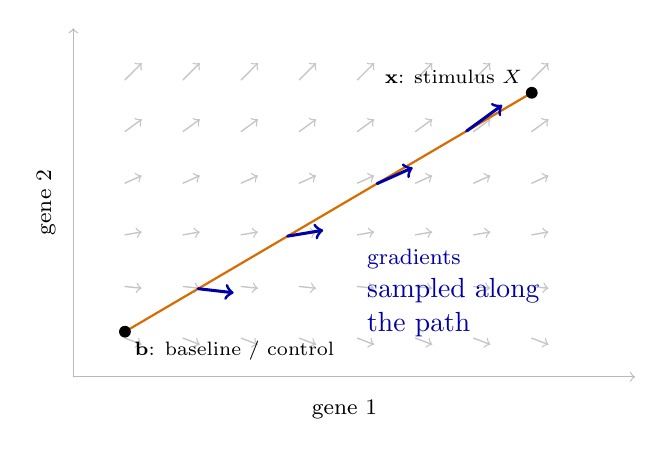
\begin{tikzpicture}[line cap=round, scale=0.82]
  \draw[->, gray!55] (0,0) -- (8.7,0);
  \draw[->, gray!55] (0,0) -- (0,5.4);
  \node at (4.2,-0.5) {\footnotesize gene 1};
  \node[rotate=90] at (-0.42,2.7) {\footnotesize gene 2};
  % gradient field grad F (grey arrows)
  \foreach \gx in {0.8,1.7,2.6,3.5,4.4,5.3,6.2,7.1}{
    \foreach \gy in {0.6,1.4,2.2,3.0,3.8,4.6}{
      \pgfmathsetmacro{\dx}{0.26}
      \pgfmathsetmacro{\dy}{0.09*(\gy-1.7)}
      \draw[->, gray!45, line width=0.5pt] (\gx,\gy) -- ++(\dx,\dy);
    }
  }
  % IG straight path: baseline -> input
  \coordinate (base) at (0.8,0.7);
  \coordinate (inp)  at (7.1,4.4);
  \draw[thick, orange!85!black] (base) -- (inp);
  \fill (base) circle (2.6pt);
  \node[below right, align=left]  at (base) {\scriptsize $\mathbf{b}$: baseline / control};
  \fill (inp) circle (2.6pt);
  \node[above left, align=right]  at (inp)  {\scriptsize $\mathbf{x}$: stimulus $X$};
  % gradients sampled along the path (blue)
  \foreach \t in {0.18,0.40,0.62,0.84}{
    \pgfmathsetmacro{\px}{0.8 + \t*(7.1-0.8)}
    \pgfmathsetmacro{\py}{0.7 + \t*(4.4-0.7)}
    \pgfmathsetmacro{\uy}{0.19*(\py-1.7)}
    \draw[->, blue!65!black, line width=1.1pt] (\px,\py) -- ++(0.55,\uy);
  }
  \node[blue!65!black, anchor=west, align=left] at (4.4,1.3) {\footnotesize gradients\\sampled along\\the path};
\end{tikzpicture}\\[2pt]
{\footnotesize (a)}
\end{minipage}\hfill
% ---------- panel (b): decompose (upper) + compare & keep (lower) ----------
\begin{minipage}[c]{0.40\textwidth}
\centering
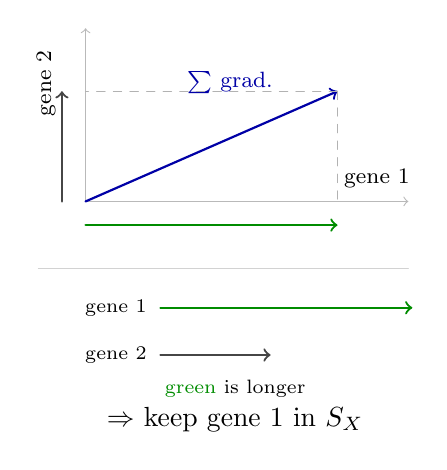
\begin{tikzpicture}[line cap=round]
  % ===== upper: decomposition (y-axis halved, sits in the upper half) =====
  \draw[->, gray!55] (0,0) -- (4.1,0);
  \draw[->, gray!55] (0,0) -- (0,2.2);
  \node[above] at (3.7,0.05) {\footnotesize gene 1};
  \node[rotate=90] at (-0.5,1.5) {\footnotesize gene 2};
  % summed gradient
  \draw[->, thick, blue!65!black] (0,0) -- (3.2,1.4);
  \node[blue!65!black, anchor=south east] at (2.5,1.25) {\footnotesize $\sum$ grad.};
  % decomposition guides
  \draw[dashed, gray!60] (3.2,1.4) -- (3.2,0);
  \draw[dashed, gray!60] (3.2,1.4) -- (0,1.4);
  % gene-1 component (green, below x-axis)
  \draw[->, thick, green!55!black] (0,-0.3) -- (3.2,-0.3);
  % gene-2 component (grey, left of y-axis)
  \draw[->, thick, gray!55!black] (-0.3,0) -- (-0.3,1.4);
  % ===== divider =====
  \draw[gray!35] (-0.6,-0.85) -- (4.1,-0.85);
  % ===== lower: lay the two components side by side, keep the longer =====
  \draw[->, thick, green!55!black] (0.95,-1.35) -- (4.15,-1.35);
  \node[left] at (0.9,-1.35) {\scriptsize gene 1};
  \draw[->, thick, gray!55!black] (0.95,-1.95) -- (2.35,-1.95);
  \node[left] at (0.9,-1.95) {\scriptsize gene 2};
  \node[align=center] at (1.9,-2.6)
    {\scriptsize {\color{green!55!black}green} is longer\\ $\Rightarrow$ keep gene 1 in $S_X$};
\end{tikzpicture}\\[2pt]
{\footnotesize (b)}
\end{minipage}
\caption{\textbf{Integrated Gradients: line integral of the gradient field, then select.}
$F$, the model's stimulus-$X$ logit, takes a whole pseudo-tube $\mathbf{x}\in\mathbb{R}^{N\times G}$
($N$ cells, $G$ genes), so attribution runs in $\mathbb{R}^{N\times G}$ and the two axes stand in
for its coordinates. The baseline $\mathbf{b}$ is the average of the control tubes' per-gene means,
weighting each tube equally, copied across the $N$ cells; the input is the stimulated tube. \textbf{(a)} Grey arrows are the gradient field $\nabla F$; Integrated
Gradients integrates it along the segment $\mathbf{b}\to\mathbf{x}$ (blue), giving attribution
$(\mathbf{x}-\mathbf{b})\odot\int_0^1\nabla F\big(\mathbf{b}+\alpha(\mathbf{x}-\mathbf{b})\big)\,d\alpha$.
\textbf{(b)} By the gradient theorem these sum to $F(\mathbf{x})-F(\mathbf{b})$; averaging over cells
gives one value per gene (top), the larger kept and the smaller dropped (bottom). The top-50 genes by
attribution form $S_X$.}
\label{fig:ig3}
\end{figure}

\rev{Figure~\ref{fig:sigselect} shows the selection step: with one attribution per gene, the genes are ranked and the top-50 (boxed) are kept as the signature $S_X$, a set of genes, while the rest are dropped.}

\begin{figure}[H]
\centering
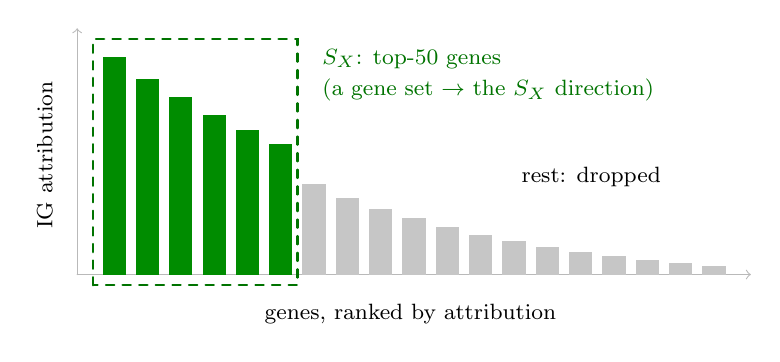
\begin{tikzpicture}[line cap=round, scale=0.92]
  % axes
  \draw[->, gray!55] (0,0) -- (9.3,0);
  \draw[->, gray!55] (0,0) -- (0,3.4);
  \node[rotate=90] at (-0.45,1.65) {\footnotesize IG attribution};
  \node at (4.6,-0.55) {\footnotesize genes, ranked by attribution};
  % kept: top genes (green)
  \foreach \i/\h in {0/3.0, 1/2.7, 2/2.45, 3/2.2, 4/2.0, 5/1.8} {
    \fill[green!55!black] ({0.35+\i*0.46},0) rectangle ({0.35+\i*0.46+0.32},{\h});
  }
  % dropped: the rest (grey), tapering off
  \foreach \i/\h in {6/1.25, 7/1.05, 8/0.9, 9/0.78, 10/0.66, 11/0.55,
                     12/0.46, 13/0.38, 14/0.31, 15/0.25, 16/0.2, 17/0.16, 18/0.12} {
    \fill[gray!45] ({0.35+\i*0.46},0) rectangle ({0.35+\i*0.46+0.32},{\h});
  }
  % box around the kept top genes
  \draw[dashed, green!45!black, thick] (0.22,-0.15) rectangle (3.04,3.25);
  \node[green!45!black, anchor=west] at (3.25,2.98) {\footnotesize $S_X$: top-50 genes};
  \node[green!45!black, anchor=west] at (3.25,2.55) {\footnotesize (a gene set $\to$ the $S_X$ direction)};
  \node[anchor=west] at (6.0,1.35) {\footnotesize rest: dropped};
\end{tikzpicture}
\caption{\textbf{Selecting the signature.} Integrated Gradients gives one attribution per gene
(Figure~\ref{fig:ig3}); ranking all genes and keeping the top-50 (green, boxed) yields the
signature $S_X$, a \emph{set} of genes, and the direction onto which cross-engagement is
measured in Section~\ref{sec:methods-direction}. The remaining genes (grey) are dropped.}
\label{fig:sigselect}
\end{figure}

Running this for every cytokine yields a set of signatures $\{S_X\}$, one per cytokine, the output of this stage and the input to the coupling and direction analysis of Section~\ref{sec:methods-direction}.

\subsection{Inferring cascade direction}
\label{sec:methods-direction}
With a signature $S_X$ now in hand for every cytokine (Section~\ref{sec:methods-signatures}), we can decide, for each pair, whether the two cytokines are coupled and, if so, whether one is upstream of the other.

\subsubsection{Engagement}
A stimulus acts differently on each cell type, so every quantity in this section is computed separately within a single cell type; the construction is repeated for each cell type, and the per-cell-type results are combined across cell types as described below. Within a fixed cell type, write $c_g$ for the expression of gene $g$ in cell $c$, let $\mathcal{C}_a$ be the cells given stimulus $a$, and let $\mathcal{C}_0$ be the control cells.
The score of a cell on a gene set $S$ is its mean expression over that set,
\[
  \sigma_S(c)=\frac{1}{|S|}\sum_{g\in S} c_g,
\]
and its average over a population of cells $\mathcal{C}$ is that population's mean signature score,
\[
  \bar\sigma_S(\mathcal{C})=\frac{1}{|\mathcal{C}|}\sum_{c\in\mathcal{C}}\sigma_S(c).
\]
The \emph{engagement} of $a$ with $b$'s signature is then $a$'s level minus the control baseline,
\[
  s(a,S_b)=\bar\sigma_{S_b}(\mathcal{C}_a)-\bar\sigma_{S_b}(\mathcal{C}_0),
\]
which quantifies ``how much of $b$'s signature appears in $a$'s response.''
The engagement $s(a,S_b)$ is computed within one cell type; writing $s_T(a,S_b)$ for its value in cell type $T$, the cross-engagement matrix combines them by the median across cell types,
\[
  M_{ab}=\operatorname*{median}_{T}\, s_T(a,S_b),
\]
taken over the cell types in which $a$ and the control have enough cells to score; since that requirement involves $a$ but not $b$, $M_{ab}$ and $M_{ba}$ may run over different cell-type sets. $M$ then holds one number per ordered pair, which the coupling score below is built from. We take the median, rather than the mean, to keep this value robust: cell types respond unevenly and some contribute extreme or noisy engagement (rare types, few cells, or non-responders), and a pair is often present in only part of the cell types, so the median reflects the typical cell type instead of being pulled by an outlying or sparsely sampled one.

Subtracting the control term is what turns a raw expression level into a measure of \emph{induction}. Signature genes are not silent at rest. On its own, $\bar\sigma_{S_b}(\mathcal{C}_a)$ therefore conflates how much stimulus $a$ actually drives $b$'s program with the level those genes sit at anyway. Subtracting their level in control cells, $\bar\sigma_{S_b}(\mathcal{C}_0)$, removes that resting baseline and leaves only the increase above rest. This matters most because $S_a$ and $S_b$ are different gene sets with different baselines: normalising each engagement to its own signature's control level puts $s(a,S_b)$ and $s(b,S_a)$ on a common footing, so that when the two are compared the difference reflects induction rather than a mismatch in resting expression between the gene sets.

\subsubsection{Coupling}
A coupled pair is one whose signatures show up in each other's response, so we score coupling by the symmetric sum $M_{ab}+M_{ba}$; a high score flags shared biology, which could be a cascade or another form of correlation.
But because many cytokines co-induce overlapping activation programs \citep{der1998identification,baysoy2023interweaved,mostafavi2016interferon,jenner2005insights,xue2014spectrum}, a broadly-engaged cytokine's signature turns up in many responses and would look coupled to everything.

\rev{We therefore keep, in place of the raw coupling, only its \emph{excess} over each cytokine's average engagement, so that a signature appearing everywhere no longer inflates every pair it takes part in.}
\rev{Collect the couplings into a matrix $C_{ab}=M_{ab}+M_{ba}$ and write $\bar C_a=\frac{1}{n-1}\sum_{b\ne a}C_{ab}$ for the mean of its $a$-th row, cytokine $a$'s average coupling to every other cytokine.}
\rev{The corrected coupling is the residual $R_{ab}=C_{ab}-\bar C_a-\bar C_b+\bar C$, with $\bar C=\frac{1}{n}\sum_a \bar C_a$ the grand mean of the couplings.}
\rev{Equivalently, $\bar C_a+\bar C_b-\bar C$ is the coupling expected for the pair from the two averages alone, and $R_{ab}$ keeps only the excess above it, the standard \emph{double-centring} of a matrix by its row, column, and grand means.}
\rev{After this correction a broadly-engaged cytokine carries a high average coupling $\bar C_a$, which is subtracted from every pair it belongs to, so it no longer registers as coupled to everything; a large $R_{ab}$ now marks coupling specific to $a$ and $b$ (Figure~\ref{fig:doublecenter}).}
\rev{Coupling and direction are the symmetric and antisymmetric combinations of the per-cell-type cross-engagements; double-centring acts only on the coupling side, so it leaves the direction call unchanged.}

\begin{figure}[H]
\centering
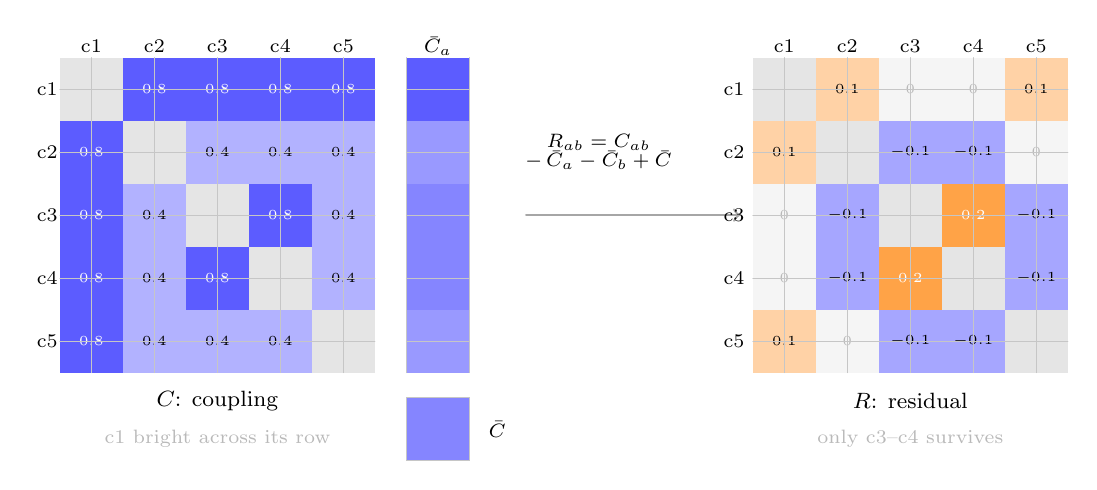
\begin{tikzpicture}[x=0.8cm,y=0.8cm,line cap=round]
  % ---------------- C: coupling matrix (before) ----------------
  % 0.8 cells: hub c1 row/column + the genuine pair c3--c4
  \foreach \i/\j in {1/2,1/3,1/4,1/5,2/1,3/1,4/1,5/1,3/4,4/3}
    {\fill[blue!64] (\j-0.5,-\i+0.5) rectangle (\j+0.5,-\i-0.5);
     \node[font=\tiny,white] at (\j,-\i) {0.8};}
  % 0.4 cells: baseline
  \foreach \i/\j in {2/3,2/4,2/5,3/2,3/5,4/2,4/5,5/2,5/3,5/4}
    {\fill[blue!30] (\j-0.5,-\i+0.5) rectangle (\j+0.5,-\i-0.5);
     \node[font=\tiny] at (\j,-\i) {0.4};}
  % diagonal: self-coupling, excluded
  \foreach \i in {1,...,5}
    \fill[gray!20] (\i-0.5,-\i+0.5) rectangle (\i+0.5,-\i-0.5);
  \draw[step=1,gray!45,thin] (0.5,-5.5) grid (5.5,-0.5);
  \foreach \j/\lab in {1/c1,2/c2,3/c3,4/c4,5/c5} \node[font=\scriptsize] at (\j,-0.32) {\lab};
  \foreach \i/\lab in {1/c1,2/c2,3/c3,4/c4,5/c5} \node[font=\scriptsize] at (0.30,-\i) {\lab};
  \node[font=\footnotesize] at (3,-5.95) {$C$: coupling};
  \node[font=\scriptsize,gray!55] at (3,-6.55) {c1 bright across its row};

  % ---------------- row means and grand mean ----------------
  \foreach \i/\p in {1/64,2/40,3/48,4/48,5/40}
    \fill[blue!\p] (6,-\i+0.5) rectangle (7,-\i-0.5);
  \draw[step=1,gray!45,thin] (6,-5.5) grid (7,-0.5);
  \node[font=\scriptsize] at (6.5,-0.32) {$\bar C_a$};
  \fill[blue!48] (6,-6.9) rectangle (7,-5.9);
  \draw[gray!45,thin] (6,-6.9) rectangle (7,-5.9);
  \node[font=\scriptsize,anchor=west] at (7.15,-6.4) {$\bar C$};

  % ---------------- operation arrow ----------------
  \draw[->,thick,gray!70] (7.9,-3) -- (11.3,-3);
  \node[font=\scriptsize,align=center] at (9.05,-2.0)
    {$R_{ab}=C_{ab}$\\[-1pt]$-\,\bar C_a-\bar C_b+\bar C$};

  % ---------------- R: residual coupling (after) ----------------
  \foreach \i/\j in {3/4,4/3}
    {\fill[orange!72] (\j+10.5,-\i+0.5) rectangle (\j+11.5,-\i-0.5);
     \node[font=\tiny,white] at (\j+11,-\i) {0.2};}
  \foreach \i/\j in {1/2,2/1,1/5,5/1}
    {\fill[orange!35] (\j+10.5,-\i+0.5) rectangle (\j+11.5,-\i-0.5);
     \node[font=\tiny] at (\j+11,-\i) {0.1};}
  \foreach \i/\j in {1/3,3/1,1/4,4/1,2/5,5/2}
    {\fill[gray!8] (\j+10.5,-\i+0.5) rectangle (\j+11.5,-\i-0.5);
     \node[font=\tiny,gray!55] at (\j+11,-\i) {0};}
  \foreach \i/\j in {2/3,3/2,2/4,4/2,3/5,5/3,4/5,5/4}
    {\fill[blue!35] (\j+10.5,-\i+0.5) rectangle (\j+11.5,-\i-0.5);
     \node[font=\tiny] at (\j+11,-\i) {$-0.1$};}
  \foreach \i in {1,...,5}
    \fill[gray!20] (\i+10.5,-\i+0.5) rectangle (\i+11.5,-\i-0.5);
  \draw[step=1,gray!45,thin] (11.5,-5.5) grid (16.5,-0.5);
  \foreach \j/\lab in {1/c1,2/c2,3/c3,4/c4,5/c5} \node[font=\scriptsize] at (\j+11,-0.32) {\lab};
  \foreach \i/\lab in {1/c1,2/c2,3/c3,4/c4,5/c5} \node[font=\scriptsize] at (11.20,-\i) {\lab};
  \node[font=\footnotesize] at (14,-5.95) {$R$: residual};
  \node[font=\scriptsize,gray!55] at (14,-6.55) {only c3--c4 survives};
\end{tikzpicture}
\caption{\rev{\textbf{Double-centring removes the hub artefact.} A five-cytokine toy example.
\emph{Left}, the coupling matrix $C_{ab}=M_{ab}+M_{ba}$: cytokine c1 is a hub, coupling
strongly (0.8) to every other cytokine, so its whole row and column are bright; c3 and c4
form a genuine specific pair (also 0.8) against a low baseline (0.4); the grey diagonal is
self-coupling, which is excluded. \emph{Middle}, each cytokine's average coupling
$\bar C_a$ (row mean) and the grand mean $\bar C$. \emph{Right}, the residual
$R_{ab}=C_{ab}-\bar C_a-\bar C_b+\bar C$: c1's high average is subtracted from its every
pair, so its row flattens to near zero and it no longer looks coupled to everything, while
c3--c4, coupled more than either partner's average predicts, remains the one strongly
positive entry (orange, above average); pairs below their average go slightly negative
(blue). The operation is symmetric, so it changes the coupling call only and leaves the
direction statistic $\mathrm{cross\_asym}$ untouched.}}
\label{fig:doublecenter}
\end{figure}

\rev{It remains to decide whether a given $R_{ab}$ is large enough to be real, and here the choice of statistical unit is decisive: pooling all cells treats thousands of correlated measurements as independent and flags almost every pair as coupled.}
\rev{The right unit is the donor: we recompute the residual once per donor, keeping the $R_{ab}^{(d)}$ from the $n_d$ donors in which both cytokines are present ($n_d\le D$, with $D\approx10$ donors in all). With $\overline{R_{ab}}=\frac{1}{n_d}\sum_d R_{ab}^{(d)}$ the mean of these residuals and $n_+=\#\{d:R_{ab}^{(d)}>0\}$ the number of them that are positive, a one-sided sign test calls the pair coupled when the mean residual is positive and the positive count exceeds a coin flip,
\[
  \overline{R_{ab}}>0 \quad\text{and}\quad p \;=\; 2^{-n_d}\sum_{k=n_+}^{n_d}\binom{n_d}{k}\;\le\;\alpha,
\]
that is, when the excess coupling is positive on average and holds in more donors than chance would give.}
\rev{The donor is the right unit because the pseudo-tubes drawn from one donor and cytokine are resampled from the same cells, correlated by construction, not independent replicates, so only the $D\approx10$ donors are genuinely independent; the test then draws its power from agreement across donors rather than from the abundance of correlated pseudo-tubes, a conservative gate that reflects real reproducibility.}


\subsubsection{Direction}
\label{sec:direction-stat}
Direction comes from the per-cell-type asymmetry: in each cell type, $\mathrm{cross\_asym}_T(a,b)=s_T(a,S_b)-s_T(b,S_a)$, and these are combined by the median across cell types, $\mathrm{cross\_asym}(a,b)=\operatorname*{median}_{T}\,\mathrm{cross\_asym}_T(a,b)$, which is large and positive exactly when $a$'s cells carry $b$'s program but not the reverse, the upstream-to-downstream signature Claim~2 predicts \rev{(Figure~\ref{fig:asymmetry})}.
Because each term needs both cytokines measured in the same cell type, this median runs only over the cell types the pair shares, unlike the coupling entries $M_{ab}$ and $M_{ba}$, which are each taken over their own cell-type set.
The quantity is antisymmetric, $\mathrm{cross\_asym}(b,a)=-\mathrm{cross\_asym}(a,b)$, so unlike the symmetric coupling sum its sign points to the upstream cytokine: the one whose cells carry more of the other's signature.
Coupling and direction are complementary: the coupling step first establishes that a pair shares biology, and $\mathrm{cross\_asym}$ then orders that shared biology from upstream to downstream.

Alongside the median we report the sign-consensus, the fraction of cell types whose own $\mathrm{cross\_asym}_T$ shares the sign of the median,
\[
  \kappa_{ab} = \frac{1}{|\mathcal{T}|}\sum_{T\in\mathcal{T}} \mathbf{1}\!\left[\operatorname{sign}\,\mathrm{cross\_asym}_T(a,b) = \operatorname{sign}\,\mathrm{cross\_asym}(a,b)\right],
\]
so a direction rests on agreement across cell types rather than on any single one.
This call is a point estimate computed on cells pooled across all donors; unlike the donor-level coupling gate it is not aggregated to the donor level, and we judge it by matching its sign against known cascades (Section~\ref{sec:methods-evaluation}).
Because a call is read from one snapshot, it points to the most likely direction of a cascade, evidence the Results confirm against known cascades, short of the intervention that would prove causation.

\subsection{Assessing the method}
\label{sec:methods-evaluation}
We cannot score the method against a ground truth of cascades, none exists, so we test it against cascades the literature has already established.
A recovered cascade has two parts to get right, that the pair is coupled at all and that its direction is correct, and we score each separately.
For coupling we report recall, the fraction of the literature-established coupled pairs the method flags, and the over-call rate, the fraction of all cytokine pairs it flags as coupled; the two together measure how well it discriminates coupled pairs, recovering the known ones without flagging most pairs indiscriminately.

The literature is all we can check against, and \textbf{it is incomplete}: a flagged pair it does not record is a candidate discovery, not a proven error, since finding new cascades is the point of the method.
This makes both extremes uninformative: a method that flagged only the already-known pairs would merely overfit the benchmark and discover nothing, while one that flagged almost every pair would recover the known ones at the cost of any selectivity.
What we look for instead is high recall together with the known cascades forming a substantial share of the flagged pairs, so that the further pairs, which engage each other much as the confirmed cascades do, are credible new candidates rather than noise.

For direction we report the fraction of the literature's directional pairs on which the sign of $\mathrm{cross\_asym}$ (Section~\ref{sec:direction-stat}) matches the documented upstream-to-downstream order.
Since a coin-flip assignment of direction would already match half the documented pairs, we judge $\mathrm{cross\_asym}$ by how far its sign-match rate rises above one-half.
As an independent check with known ground truth, we apply $\mathrm{cross\_asym}$ to simulated cells carrying a planted cascade, where the correct direction is set in advance and can be compared against the statistic's call.

Throughout, we require the findings to hold across independent training seeds and across separate datasets, so that neither the coupling nor the direction conclusions rest on a single run.

\section{Results}
\label{sec:results}
% >>> write here

\subsection{Frozen versus unfrozen encoder}
\label{res:unfreeze}
% >>> write here

\section{Discussion}
\label{sec:discussion}
% >>> write here

\section{Limitations}
\label{sec:limitations}
% >>> write here

\section{Conclusion and Future Work}
\label{sec:conclusion}
% >>> write here

% ----------------------------------------------------------------------------
%  BACK MATTER
% ----------------------------------------------------------------------------
\newpage
\bibliography{references}

\appendix
\section{Supplementary Material}
\label{app:supplementary}

\subsection{Cell identity dominates single-cell variation}
\label{app:umap}

\begin{figure}[H]
\centering
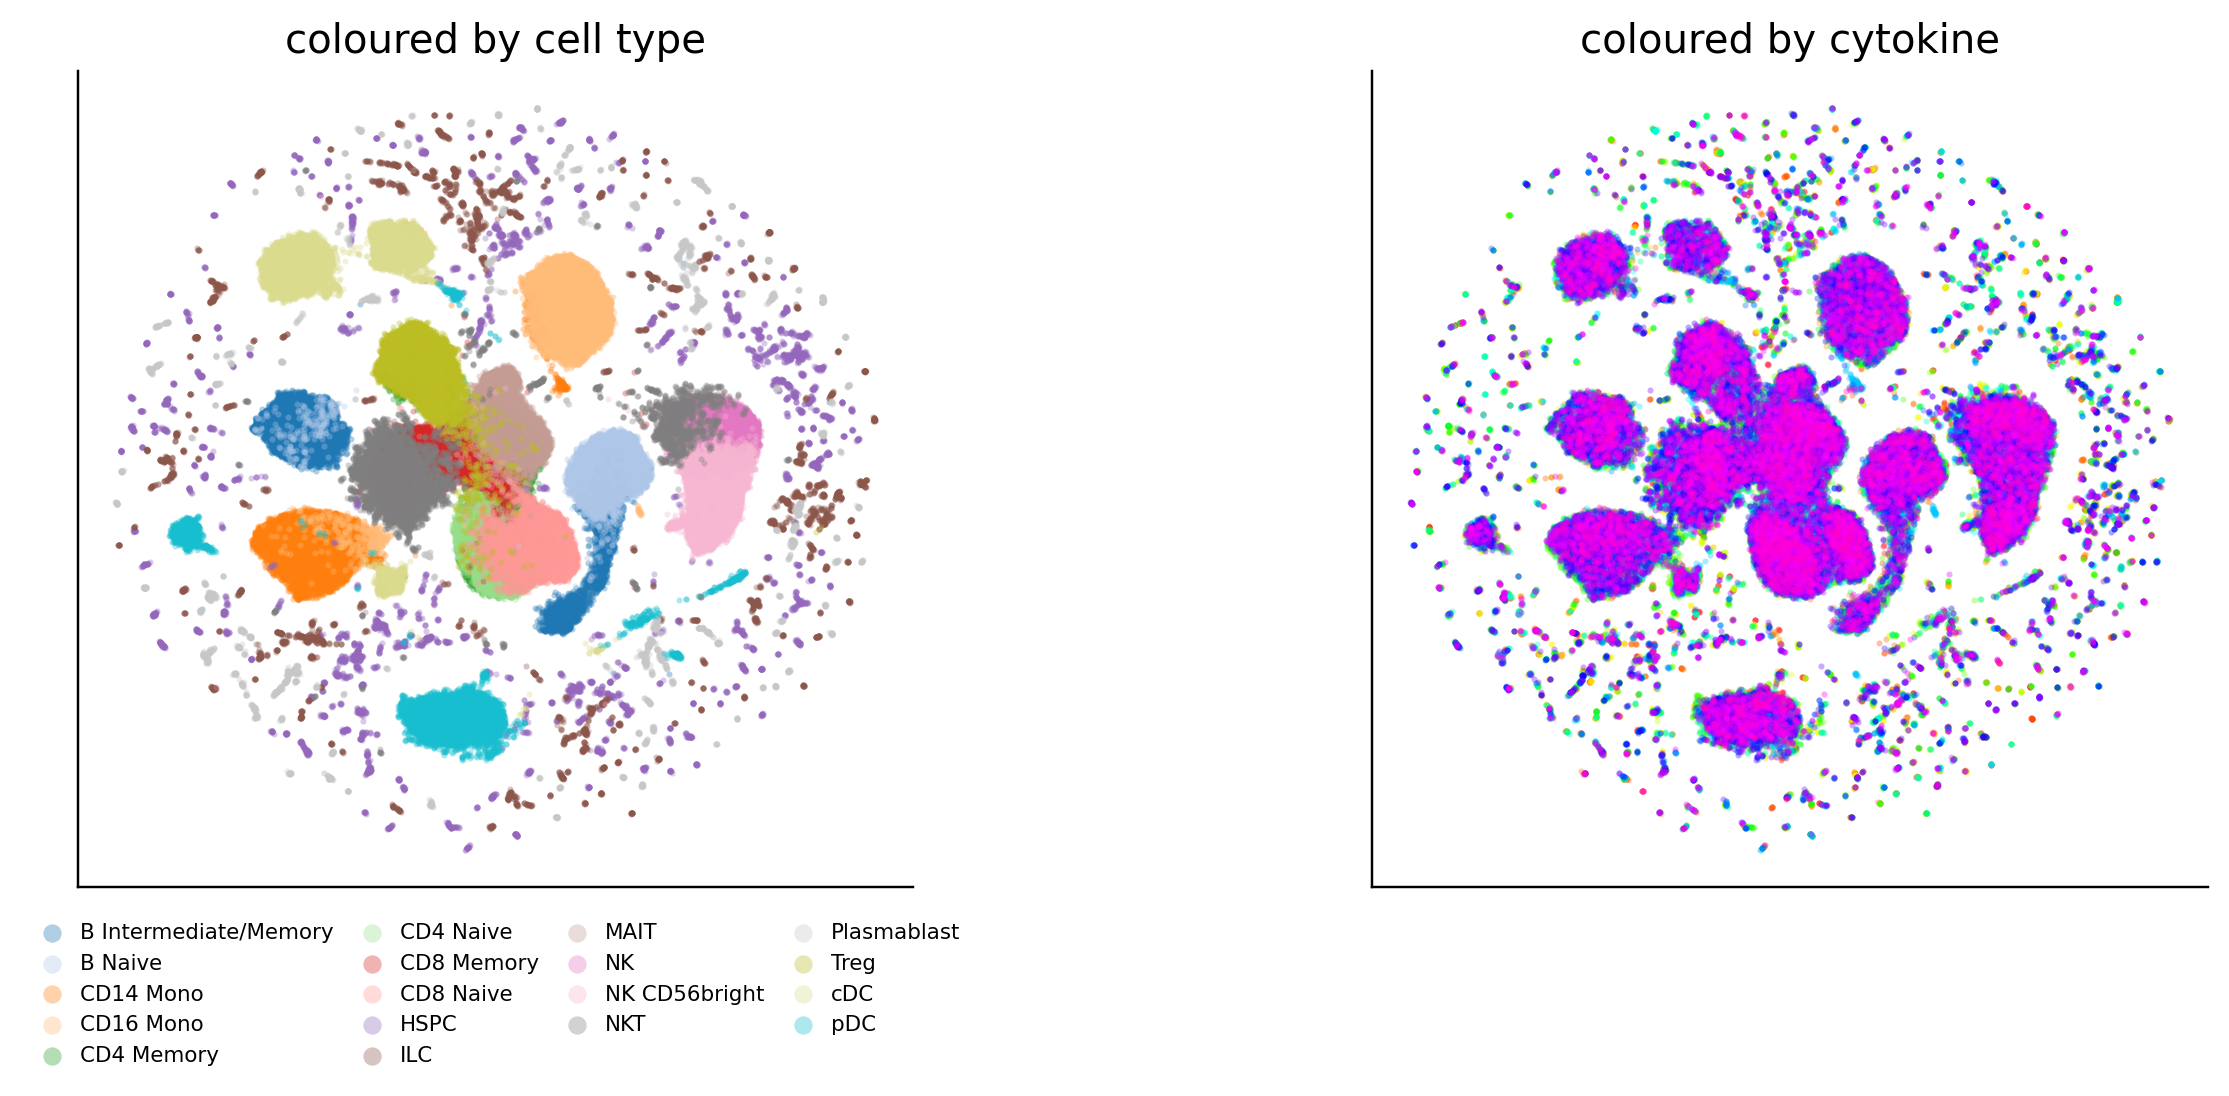
\includegraphics[width=\textwidth]{umap.png}
\caption{\textbf{Cell identity, not cytokine, organises the single-cell landscape.} Two-dimensional UMAP of all cells from a single donor (three pseudo-tubes per cytokine), computed from the log-normalised high-variable-gene expression. \emph{Left}, points coloured by cell type; \emph{right}, the same points coloured by the applied cytokine. Cells separate into well-defined islands by cell type, while cytokines are intermixed within those islands, showing that cell identity, rather than the applied cytokine, is the dominant axis of transcriptional variation. This motivates pretraining the encoder on cell type (Section~\ref{sec:sig-architecture}).}
\label{fig:umap}
\end{figure}

\subsection{Efficient training with a frozen encoder}
\label{app:efficiency}
Because the encoder is frozen in the second training stage (Section~\ref{sec:sig-training}), each cell is mapped to the same embedding at every step of the optimisation. That embedding can therefore be computed once per pseudo-tube and reused, so only the attention and classifier, a small fraction of the model, are evaluated during the repeated training steps. Since the encoder has no stochastic components, this caching leaves the trained model and its extracted signatures unchanged, and is purely a speed-up. \todo{expand: fuller description of the embedding cache}

\end{document}
